We could m optimize using Waw


\section{Outline}


Phase 1. Pick all vertices whose neighborhood cannot be dominated by $3$
vertices. $\rightarrow D_1$. 

\bigskip
Phase 2. For every $v$, if there is $w\neq v$ with $N(v)\cap N[w]\geq 11$, 
then pick $w$. $\rightarrow D_2$.

------------------------------------------------------

Reworked up until this point!

$D_1 = \{ v \> | \> N(v) \text{ not dominated by 3 vertices} \}$

$|D_1 \setminus D| \leq 3\gamma$

$D_2 = \{v|\exists v_0 \neq v \land v_0 \notin D_1 \land v \notin D_1 \land (N(v_0) \land N[v] \geq 6)\}$

\begin{lemma}
$|D_2 \setminus D | \leq 7 \gamma$

$|\{v_0, v \> | \> v \in D_2 \land v \notin D \land v_0 \notin D \}| \leq \gamma$

$|\{ v_0, v \> | \> v \in D_2 \land v_0 \in D\} |  \leq 6 \gamma$
\end{lemma}

\begin{lemma}
$D_3 = \{ v \> | \> N[v] \land (D_1 \lor D_2) = \varnothing \} $

$|D_3 \setminus \gamma \> | \leq 16 \gamma$
\end{lemma}
















------------------------------------------------------
\begin{lemma}
$|D_2\setminus D|\leq 4\gamma$.
\end{lemma}
\begin{proof}
For $v\in D$ we can have $3$ vertices, hence at most $3\gamma$. 

If $v\not\in D$ and $w\neq v$ with $N(v)\cap N[w]\geq 11$ and $w\not\in D$,
excluding $w$ will result in 10 vertices which have to be dominated. 
Assume the 10 vertices can be domminated by three vertices $v_1, v_2, v_3$.
They dominate 3 vertices by themself meaning they have to dominate 7 others, 
thus resulting in one vertex dominating at least 3 others. 
As a result $v, w, v_i$ connect to 3 other vertices resulting in a $K_{3,3}$, therefore needing at least 4 vertices for every neighborhood of 11.
%then the face spanned by $v,w$ and the two outer boundary
%vertices contains (at least) $2$ elements of $D$ that are unique
%for this face. By Euler's formula we have $n=2-f+m$. Here, every face
%has at most $4$ edges, so $n\leq 2+3f\leq 2+\frac{3}{2}\gamma\leq 2\gamma$. 
\end{proof}

Now carry out the analysis as Wawrzyniak~\cite{wawrzyniak2014strengthened}
with the observation that every double star has size at most $11$. This should
lead to additional $23\gamma$ added vertices. In total we would get
$(3+5+23+1)\gamma=32\gamma$ vertices in the dominating set. Maybe
the analysis of Wawrzyniak~\cite{wawrzyniak2014strengthened} can be
improved even more. 

In the $C_4$-free case for $v\in V(G)$ there is no $w$ with $N(v)\cap N[w]\geq 3$. 
In case of girth $4$ there is even no $w$ with $N(v)\cap N[w]\geq 2$. 

------------------ 

Old lemmas that may not be needed anymore. 

\begin{lemma}
There are at most $3\gamma$ vertices not in $D$ whose neighborhood cannot
be dominated by $3$ other vertices from $D$. 
\end{lemma}

$\rightarrow$ Set $D'$ that cannot be computed, but it helpful for the analysis. 

\begin{lemma}
If $v\not\in D'$ and there is $w\neq v$ with $N(v)\cap N[w]\geq 11$, 
then $w\in D$. 
\end{lemma}



\begin{corollary}
$|D_2\setminus D|\leq 12\gamma$ ($|D'\cup D|\cdot 3$). 
\end{corollary}


\section{Preliminaries}

In this section we fix our notation and prove some basic lemmas
required for the algorithm. We use standard notation from graph
theory and refer to the literature for extensive background. For an
undirected and simple graph~$G$ we denote by $V(G)$
the vertex set and by $E(G)$ the edge set of $G$. We also refer
to the literature, for the
formal definition of the LOCAL model of distributed computing.

A graph~$H$ is a minor of a graph~$G$, written~$H\minor G$, if
there is a set \mbox{$\{G_v :v\in V(H)\}$} of pairwise vertex disjoint and
connected subgraphs
$G_v\subseteq G$ such that if~$\{u,v\}\in E(H)$, then there is an edge
between a vertex of~$G_u$ and a vertex of~$G_v$. We call $V(G_v)$ the
\emph{branch set} of $v$ and say that it is
\emph{contracted} to the vertex~$v$.
%If $G_1,\ldots, G_k\subseteq V(G)$
%are pairwise vertex disjoint and connected subgraphs of $G$, then we write
%$G/G_1/\ldots/G_k$ for the minor obtained by contracting the subgraphs~$G_i$ (observe that the order of contraction does not matter as the
%$G_i$'s are vertex disjoint).

For a non-negative integer~$r$, a graph
$H$ is an \emph{$r$-shallow minor} of $G$, written
$H\minor_r G$, if there is a set~$\{G_v : v\in V(H)\}$ of pairwise
vertex disjoint connected subgraphs
$G_v\subseteq G$ of radius at most $r$ such that if~$\{u,v\}\in E(H)$,
then there is an edge between a vertex of~$G_u$ and a vertex of~$G_v$.
Observe that a $0$-shallow minor of $G$ is just a subgraph of $G$.

We write $\nabla_r(G)$ for $\max_{H\minor_r G}|E(H)|/|V(H)|$. Observe
that $\nabla_0(G)$ denotes the maximum average edge density of $G$
and $2\nabla_0(G)$ bounds the degeneracy of~$G$, which is defined
as $\max_{H\subseteq G}\delta(H)$. Here, $\delta(H)$ denotes
the minimum degree of~$H$.
%
A class~$\Cc$ of graphs has \emph{bounded expansion} if there is a function
$f:\N\rightarrow\N$ such that $\nabla_r(G)\leq f(r)$ for all graphs $G\in \Cc$.
This is equivalent to demanding that the degeneracy of each $r$-shallow minor
of $G$ is functionally bounded by~$r$.

We write~$K_{s,t}$ for the complete bipartite
graph with partitions of size~$s$ and~$t$, respectively. Observe that
$K_{t,t}$ has $2t$ vertices and $t^2$ edges, hence, if
\mbox{$\nabla_0(G)< t/2$}, then $G$ excludes $K_{t,t}$ as a subgraph.

For a graph $G$ and $v\in V(G)$ we write $N(v)=\{w~:~\{v,w\}\in E(G)\}$
for the \emph{open neighborhood} of $v$ and $N[v]=N(v)\cup\{v\}$ for
the \emph{closed neighborhood} of~$v$. For a set $A\subseteq V(G)$ let
$N[A]=\bigcup_{v\in A}N[v]$. We write $N_r[v]$ for the set
of vertices at distance at most $r$ from a vertex $v$.
A dominating set in a graph~$G$ is a set
$D\subseteq V(G)$ such that $N[D]=V(G)$. We write $\gamma(G)$ for
the size of a minimum dominating set of $G$. For $W\subseteq V(G)$
we say that a set $Z\subseteq V(G)$ \emph{dominates} or \emph{covers} or
is a \emph{cover} of $W$ if $W\subseteq N[Z]$.
Observe that we do not
require $Z\cap W=\emptyset$ as Czygrinow et al.\ do for covers.

\smallskip
The following lemma is one of the key lemmas used for the algorithm. It goes back to~\cite{lenzen2013distributed}.

\begin{lemma}\label{lem:neighborhood-dom1}
Let $G$ be a graph. Then there are less than $2\gamma(G)$ vertices $v$ with the property that $N(v)$ cannot be dominated by at most $2\nabla_1(G)$ vertices different from $v$.
\end{lemma}
\begin{proof}
Let $\gamma=\gamma(G)$ and $\nabla_1=\nabla_1(G)$ and assume that there are $2\gamma$ such vertices $a_1,\ldots,a_{2\gamma}$. We proceed towards a contradiction.
  Let $\{d_1,\ldots,d_\gamma\}$ be a minimum dominating set. At least $\gamma$ of the $a_i$'s are not in this dominating set. We can hence assume w.l.o.g.~that $\{a_1,\ldots,a_{\gamma}\}$ and $\{d_1,\ldots,d_\gamma\}$ are two disjoint sets of vertices.

We build a $1$-shallow minor $H$ of the graph $G$ with the following $2\gamma$ branch sets. For every $i\le \gamma$, we have a branch set
$A_i=\{a_i\}$ and a branch set $D_i=N[d_i]\setminus (\{a_1,\ldots, a_\gamma\}\cup \bigcup_{j<i}N[d_j] \cup \{d_{i+1},\ldots, d_\gamma\})$.
We call the associated vertices of $H$ $a_1',\ldots, a_\gamma',d_1',\ldots,
d_\gamma'$.

Since $\{d_1,\ldots, d_\gamma\}$ is a dominating set of $G$ and by assumption on $N(a_i)$, we have that in $H$, every $a'_i$ is connected to at least $2\nabla_1+1$ of the $d'_i$.
  We therefore have that $|V_H|=2\gamma$ and $|E_H| \ge \gamma(2\nabla_1+1)$, hence $|E_H|> |V_H|\nabla_1$, a~contradiction.
\end{proof}

\hrulefill
%%%%%%%%%%%%%%%%%%%%%%%%%%%%%%%%%%%%%%%%%%%%%%%%%%%%%%%%%%%%%%%%%%%%%%%%%%%%%%%%
% Worked up until here %
%%%%%%%%%%%%%%%%%%%%%%%%%%%%%%%%%%%%%%%%%%%%%%%%%%%%%%%%%%%%%%%%%%%%%%%%%%%%%%


Note that we cannot locally determine the number $\nabla_1(G)$.
We must hence assume that it is given with the input. Observe that
similarly, the algorithm of Czygrinow et al.\ works with the assumption
that the input excludes a complete graph with $t$ vertices as a topological
minor. This implies a bound on the edge density of topological minors
in $G$, which can be seen as being given with the input.

The algorithm proceeds in three phases. The first phase is
based on \cref{lem:neighborhood-dom1} as follows.
In the LOCAL model we can learn the distance-$2$
neighborhood~$N_2[v]$ of every vertex $v$ in $2$ rounds,
and then locally check
whether~$N(v)$ can be domi\-nated by at most $2\nabla_1(G)$
vertices.

\begin{tcolorbox}
% \fbox{
% \begin{minipage}{0.9\linewidth}
We let $D_1$ be the set of all vertices that do not have this
property. By \cref{lem:neighborhood-dom1}
we have $|D_1|\leq 2\gamma(G)$. We remove $D_1$ from the
graph and mark all its neighbors as dominated in one additional round.
% \end{minipage}
% }
\end{tcolorbox}


In the following we fix a graph $G$ and we assume that $N(v)$ can be
dominating by at most $2\nabla_1(G)$ vertices different from $v$
for all $v\in V(G)$. We write $\nabla_1$ for~$\nabla_1(G)$ and
we let $t\leq 2\nabla_0(G)+1$ be the smallest positive integer
 such that~$G$ excludes
$K_{t,t}$ as a subgraph. Note that this number is not required
as part of the input. We let $k\coloneq 2\nabla_1$.

\begin{example}
  A planar $n$-vertex graph has at most $3n-6$ edges. A minor of a
  planar graph is again planar, hence for planar graphs $G$ we have $\nabla_r(G) \leq 3$ for all $r\geq 0$ and $k=2\nabla_1(G)\leq 6$.
\end{example}

We also fix a minimum dominating set $D$ of $G$
of size~$\gamma$.
% In the following, when we speak of ``almost all vertices'', we mean all but at most~$c\gamma$ vertices for some
% constant $c$. This is again motivated by the argument that adding
% any~$c\gamma$ vertices
% to the dominating set will still give a constant factor approximation.
The following lemma is proved exactly as \cref{lem:neighborhood-dom1}.

\begin{lemma}\label{lem:neighborhood-dom2}
There are less than $2\gamma$ vertices $v$ with the property
that $N(v)$ cannot be dominated by at most $2\nabla_1$ vertices
from $D$ and different from $v$.
\end{lemma}

Unfortunately, we cannot determine these vertices locally, as it requires
know\-ledge of $D$, however, this structural property is very useful for
our further argumentation.

\begin{tcolorbox}
% \begin{minipage}{0.92\linewidth}
Denote by $\hat D$ the set of all vertices $v$
whose neighborhood cannot be dominated
by $2\nabla_1$ vertices of $D$ different from $v$.
Let $D'=D\cup \hat D$.
% \end{minipage}
\end{tcolorbox}

According to %\cref{lem:neighborhood-dom1} and
\cref{lem:neighborhood-dom2}, $D'$ contains at most
%$(1+4\nabla_1)\gamma$ vertices.
$3\gamma$ vertices.
% \alex{shouldn't we simply add $v$ in $D'$? We then get that $|D'|\le 3\gamma$.\\
%   $\gamma$ for $D$, and at most $2\gamma$ such vertices.}
Let us stress that~$D'$ will never be computed by our LOCAL algorithm. We only use
its existence in the correctness proofs.

\smallskip
We can apply these
lemmas to obtain a constant factor approximation for a dominating
set only if $\nabla_1(G)$ is bounded by a constant. For example in graphs of bounded degeneracy in general the number of vertices that dominate the
neighborhood of a vertex can only be bounded by $\gamma(G)$.
Hence, the approach based on covers and pseudo-covers that is employed
in the following cannot be extended to degenerate  graph classes.

\begin{example}
Let $G(\gamma,m)$ be the graph with vertices $v_i$ for $1\leq i\leq \gamma$,
$w^j$ for $1\leq j\leq m$ and $s_i^j$ for $1\leq i\leq \gamma, 1\leq j\leq m$.
We have the edges $\{v_1, w^j\}$ for $1\leq j\leq m$, hence $v_1$
dominates all $w^j$. We have the edges $\{w^j, s_i^j\}$ for all $1\leq i\leq \gamma,
1\leq j\leq m$, hence, the $s_i^j$ are neighbors of $w^j$. Finally,
we have the edges $\{v_i, s_i^j\}$, that is, $v_i$ dominates the $i$th
neighbor of $w_j$. Hence, for $m>\gamma$,
$G(\gamma, m)$ has a dominating set of size
$\gamma$ and $m$ vertices whose neighborhood can be dominated
only by $\gamma(G)$ vertices. \cref{lem:neighborhood-dom1} implies
that $\gamma < 2\nabla_1$, and as we can choose~$m$ arbitrary
large, we cannot usefully apply \cref{lem:neighborhood-dom1}.
Furthermore, $G(\gamma,m)$ is
\mbox{$2$-degenerate}, showing that these methods cannot be applied on
degenerate graph classes.

\begin{center}
  \begin{figure}
    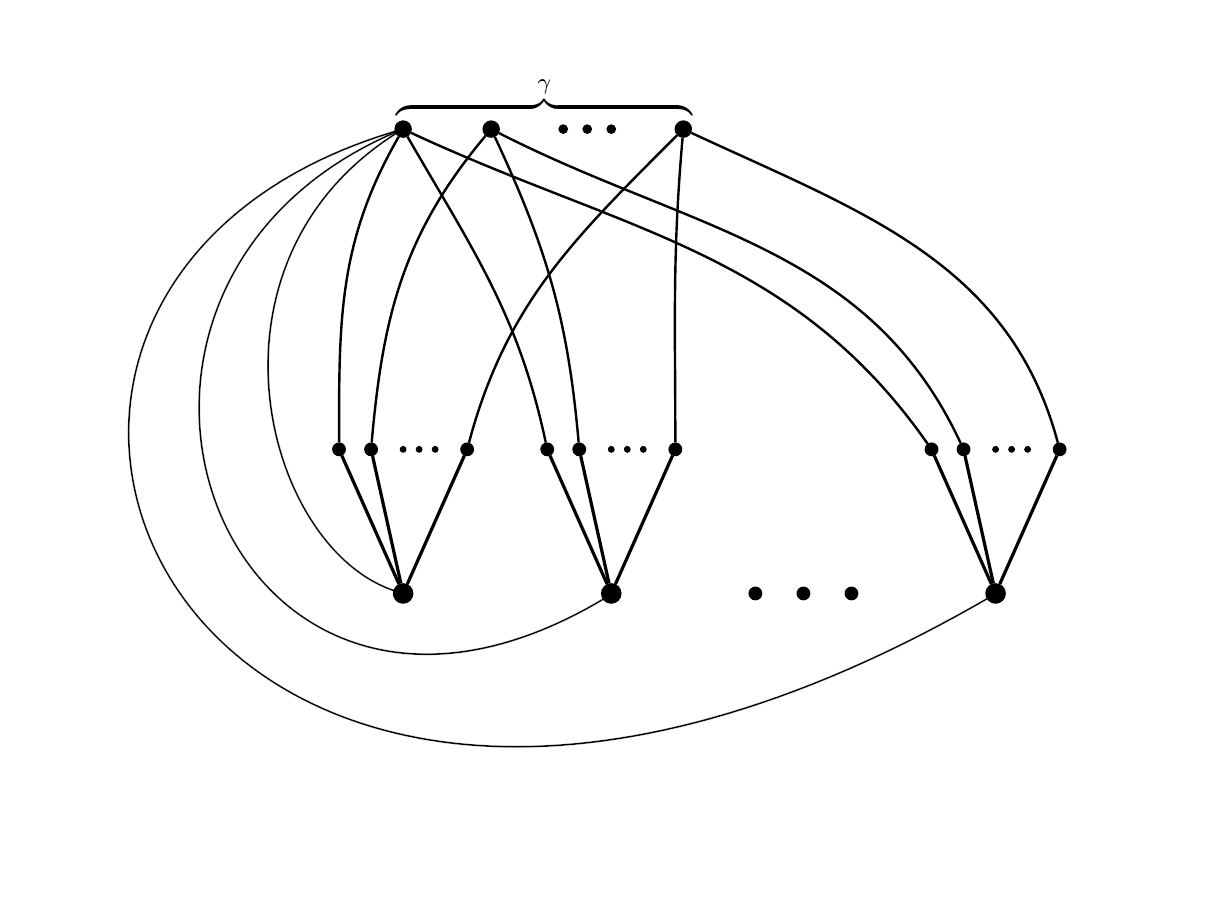
\includegraphics[scale=0.3]{ds1.png}
    \caption{ A $2$-degenerate graph where for many $v\in V(G)$ the set $N(v)$ can only be dominated by at least $\gamma$ vertices different from $v$. }
  \end{figure}
\end{center}
\end{example}


%
\section{Covers and pseudo-covers}

Intuitively, the vertices from a cover of a set $W$ can
take different roles. A few vertices of a cover may cover almost the
complete set $W$, while a few others are only there to cover what was
left over. The key observation of Czygrinow et al.\ is that in classes that
exclude some~$K_{t,t}$ as a subgraph, there can only be few of such
high degree covering vertices, while there can be arbitrarily many vertices
that cover at most $t-1$ vertices of~$W$ (the same vertices can be covered
over and over again). This observation can be applied recursively and is
distilled into the following two definitions. Recall that by the processing
carried out in the first phase of the algorithm
we know that every neighborhood $N(v)$ can be covered by $k=2\nabla_1$ vertices different from $v$.
% For the rest of this article we fix
% $\alpha\coloneqq 1/k$, $\ell=8\nabla_1/\alpha^2+1=4k^3+1$ and $q=4k^4$.
% These constants will be needed in the following definitions of pseudo-covers
% and domination sequences.
We recall all fixed parameters for easy to find reference.

\bigskip
\begin{tcolorbox}
\begin{tabular}{l l}
- $G$ & :~ fixed graph. \\
- $\gamma$ & :~ $\gamma(G)$.\\
- $\nabla_1$ & :~ $\nabla_1(G)$. \\
- $t$ & :~ smallest integer such that $G$
excludes $K_{t,t}$ as a subgraph\\
- $D_1$ & :~ defined and computed in \cref{lem:neighborhood-dom1}.\\
- $D$ & :~ fixed dominating set of $G$ of size $\gamma$ (not computed).\\
- $\hat{D}$ & :~ defined in \cref{lem:neighborhood-dom2} (not computed).\\
- $D'$ & :~ $D \cup \hat{D}$ (not computed).
\end{tabular}
\end{tcolorbox}

% For the rest of this article we fix
% $\alpha\coloneqq 1/k$, $\ell=8\nabla_1/\alpha^2+1=4k^3+1$ and $q=4k^4$.
% These constants will be needed in the following definitions of pseudo-covers
% and domination sequences.
% We also fix the following constants to follow the presentation
% of~\cite{czygrinow2018distributed}.

Following the presentation of~\cite{czygrinow2018distributed}, we name and fix
these constants for the rest of this article.

\begin{tcolorbox}
\begin{tabular}{l l}
- $k$       & $\coloneqq~ 2\nabla_1$.\\
- $\alpha$  & $\coloneqq~ 1/k$.\\
- $\ell$    & $\coloneqq~ 8\nabla_1/\alpha^2+1=4k^3+1$.\\
- $q$       & $\coloneqq~ 4k^4$.
\end{tabular}
\end{tcolorbox}


\begin{definition}
A vertex $z\in V(G)$ is \emph{$\alpha$-strong} for a vertex set $W\subseteq V(G)$ if $|N[z]\cap W|\geq \alpha|W|$.
\end{definition}

The following is the key definition by Czygrinow et al.~\cite{czygrinow2018distributed}.

\begin{definition}
A \emph{pseudo-cover} (with parameters $\alpha, \ell, q, k$)
of a set $W\subseteq V(G)$ is a
sequence $(v_1,\ldots, v_m)$ of vertices
such that  for every $i$ we have
\begin{itemize}
\item $|W\setminus \bigcup_{j\le m}N[v_j]|\leq q$,
\item $v_i$ is $\alpha$-strong for $W\setminus\bigcup_{j<i}N[v_j]$,
\item $|N[v_i]\cap (W\setminus\bigcup_{j<i} N[v_j])|\geq \ell$,
\item $m\leq k$.
\end{itemize}
\end{definition}
Intuitively, all but at most $q$ elements of the set $W$ are covered by the $(v_i)_{i\le m}$.
Additionally, each element of the pseudo-cover dominates both an
$\alpha$-fraction of what remains to be dominated, and at least $\ell$ elements.
Note that with our choice of constants, if there are more than $q$ vertices not
covered yet, any vertex that covers an $\alpha$-fraction of what remains also
covers at least $\ell$ elements.


The next lemma shows how to derive the existence of pseudo-covers from
the existence of covers.

\begin{lemma}\label{lem:cover-to-pseudo-cover}
Let $W\subseteq V(G)$ be of size at least
$q$ and let~$Z$ be a cover of $W$ with~$k$ elements.
There exists an ordering of the vertices of $Z$ as $z_1,\ldots, z_k$
and $m\leq k$ such that $(z_1,\ldots, z_m)$ is a pseudo-cover of $W$.
\end{lemma}
\begin{proof}
 We build the order greedily by induction. We order the elements by neighborhood size, while removing the neighborhoods of the previously ordered vertices. More precisely, assume that $(z_1,\ldots,z_i)$ have been defined for \mbox{some~$i\ge 0$}. We then define $z_{i+1}$ as the element that maximizes $|N[z] \cap (W \setminus \bigcup_{j\le i}N[z_j])|$.

 Once we have ordered all vertices of $Z$, we define $m$ as the maximal integer not larger than $k$ such that for every $i \le m$ we have:
 \begin{itemize}
   \item $z_i$ is $\alpha$-strong for $W\setminus\bigcup_{j<i}N[z_j]$, and
   \item $|N[z_i] \cap (W \setminus \bigcup_{j\le i}N[z_j])| \ge \ell$.
 \end{itemize}

This made sure that $(z_1,\ldots, z_m)$ satisfies the last 3 properties of a
 pseudo-cover of $W$. It only remains to check the first one.
 To do so, we define $W' \coloneq W \setminus\bigcup_{i\le m}N[z_i]$. We want to prove
 that $|W'| \le q$. Note that because $Z$ covers~$W$, if $m=k$ we
 have $W'=\emptyset$ and we are done. We can therefore assume
 that $m<k$ and $W'\neq \emptyset$. Since $Z$ is a cover of $W$,
 we also know that $(z_{m+1},\ldots z_k)$ is a cover of $W'$,
 therefore there is an element in $(z_{m+1},\ldots z_k)$ that
 dominates at least a $1 / k$ fraction of $W'$. Thanks to the
 previously defined order, we know that~$z_{m+1}$ is such element.
 Since $\alpha = 1/k$, it follows that~$z_{m+1}$ is $\alpha$-strong
 for $W'$.
 This, together with the definition of $m$, we have that $|N[z_i] \cap (W \setminus \bigcup_{j\le i}N[z_j])| < \ell$ meaning that $|N[z_{m+1}] \cap W'| < \ell$. This implies that $|W'|/k < \ell$. And since $\ell = q/k$, we have $|W'|<q$.
%
  Hence, $(z_1,\ldots, z_m)$ is a pseudo-cover of $W$.
\end{proof}

%We will apply the pseudo-covers to neighborhoods
%of vertices.

While there can exist unboundedly many covers for a set $W\subseteq V(G)$,
the nice observation of Czygrinow et al.\ was that the number of
pseudo-covers is bounded whenever the input graph excludes some
biclique $K_{s,t}$ as a subgraph. We do not state the result in this
generality, as it leads to enormous constants. Instead, we focus on the
case where small covers exist, that is, on the case where~$\nabla_1(G)$
is bounded and optimize the constants for this case.

\begin{lemma}\label{lem:num-high-degree}
Let $W\subseteq V(G)$ of size at least $8\nabla_1 / \alpha^2$.
Then there are at most $4\nabla_1/\alpha$ vertices that are
$\alpha$-strong for $W$.
\end{lemma}
\begin{proof}
  Assume that there is such a set $W$ with at least $c\coloneq 4\nabla_1 /\alpha$ vertices that are $\alpha$-strong for $W$.
  We build a $1$-shallow minor $H$ of the graph $G$ with $|W|$ branch sets.
  Each branch set is either a single element of $W$, or a pair $\{w,a\}$, where $w$ is in $W$ and $a$ is an $\alpha$-strong vertex for $W$, connected to $w$, and that is not in $W$. This is obtained by iteratively contracting one edge of an $\alpha$-strong vertex with a vertex of $W$. This is possible because $\alpha |W|>c$, so during the process and for any \mbox{$\alpha$-strong} vertex we can find a connected vertex in $W$ that is not part of any contraction.

  Once this is done, we have that $|V_H|=|W|$. For the edges, each of the \mbox{$\alpha$}-strong vertices can account for $\alpha |W|$ many edges. We need to subtract~$c^2$ from the total as we do not count twice an edge between two strong vertices. Therefore $|E_H| \ge c\alpha |W| - c^2$. Note also that because $|W| \ge 8\nabla_1 / \alpha^2$, we have that $ 2\nabla_1\ge (4\nabla_1)^2 / (\alpha^2|W|)$. All of this together leads to:

  $$\frac{|E_H|}{|V_H|} \ge \frac{c\alpha |W| - c^2}{|W|} \ge 4 \nabla_1 - \frac{(4\nabla_1)^2}{\alpha^2|W|} \ge 4\nabla_1 - 2\nabla_1 > \nabla_1 $$

  This contradicts the definition of $\nabla_1$.
\end{proof}

This leads quickly to a bound on the number of pseudo-covers.

\begin{lemma}\label{lem:num-pseudo-covers}
For every $W\subseteq V(G)$ of size at least $\ell$, the number of pseudo-covers is bounded by $2(4\nabla_1(G)/\alpha)^k$.
\end{lemma}

The proof of the lemma is exactly as the proof of Lemma~7 in the
presentation of Czygrinow et al.~\cite{czygrinow2018distributed},
we therefore refrain from repeating it here.

%
%Having previous decided to fix $K$ and $\alpha$, \cref{lem:num-pseudo-covers}
%yields the following handy corollary.
%\begin{corollary}\label{cor:num-pseudo-covers}
%  Let $G$ be a graph. Fixe $k\coloneq 2\nabla_1(G)$, and then define
%  $\alpha = 1/k$, $K=k$, $\ell =4k^3+1$, and $q:= 4k^4$.
%  Then for every $W\subseteq V(G)$ of size at least $\ell$, the number of
%  $(\alpha,q,\ell,K)$-pseudo-covers of $W$
%  is bounded by $2(2k^2)^k$.
%\end{corollary}

% \textcolor{blue}{
% \begin{example} Let $G$ be a planar graph. We can strongly optimize
% the construction. For $\alpha>0, \ell\geq 8, q\geq 0$ and
% $K\leq 6$ the number of vertices appearing in any $(\alpha, q,\ell, K)$-pseudo-cover
% of $N(v)$ for a vertex $v$ is at most $7$.
% The neighborhood $N(v)$ is dominated by $v$ and also by
% at most $6$ vertices from $D'$. Then there does not exist
% a further vertex that dominates at least $8$ vertices of
% $N(v)$ as $G$ is planar. PROOF+PICTURE.
% \end{example}
% }

\begin{tcolorbox}
We write $\Tt(v)$ for the set of all pseudo-covers
of $N(v)$ and $\Pp(v)$ for the set of all vertices that appear in a
pseudo-cover of $N(v)$.
\end{tcolorbox}



\begin{corollary}\label{cor:nb-dominators}
For every $v\in V(G)$ with $|N(v)|> \ell$, we have
  $|\Tt(v)|\le 2(2k^2)^k$ and $|\Pp(v)|\le 2k(2k^2)^k\le (2k)^{2k+1}$.
\end{corollary}


\section{Finding dominators}


Recall that by \cref{lem:neighborhood-dom2} for every $v\in V(G)$ we can
cover $N(v)$ with at most~$k$ vertices from $D'$.
To first gain an intuitive understanding of the second phase of the
algorithm, where we construct a set $D_2\subseteq V(G)$, let us consider the
following iterative procedure.

Fix some $v\in V(G)$. Let $v_1=v$ and $B_1\coloneqq N(v)$
and assume $|B_1|\geq k^{t-1}(2t{-}1)$. We consider $s$
vertices $v_1,v_2\ldots, v_s$ as follows.
Choose as~$v_2$ an arbitrary vertex different from $v_1$
that dominates at least $k^{t-2}(2t-1)$ vertices of~$B_1$, that is,
a vertex that satisfies $|N[v_2]\cap B_1|\geq k^{t-2}(2t-1)$.
Note that any vertex~$v_2$ that dominate a $1/k$-fraction of $B_1$ can
be such vertex, i.e.~it is enough for $v_2$ to be $\alpha$-strong for $B_1$.

Let $B_2\coloneqq N(v_2)\cap B_1$. Observe that we consider
the open neighborhood of $v_2$ here, hence $B_2$ does
not contain $v_2$. Hence, $|B_2|\geq k^{t-2}(2t-1)-1\geq
k^{t-2}(2t-2)$.
We continue to choose vertices $v_3,\ldots$ inductively
just as above. That is, if the vertices $v_1,\ldots,v_i$ and sets
$B_1,\ldots, B_i\subseteq V(G)$ have been defined, we choose
the next vertex $v_{i+1}$ as an arbitrary vertex not in $\{v_1,\ldots,
v_i\}$ that dominates
at least $k^{t-i-1}(2t-i)$ vertices of $B_i$, that is, a vertex with
$|N[v_{i+1}]\cap B_i| \ge k^{t-i-1}(2t-i)$ and let
$B_{i+1}\coloneqq N(v_{i+1})\cap B_i$, of size at least
$k^{t-i-1}(2t-i-1)$.



\begin{lemma}\label{lem:sequence}
Assume $|N(v)|\geq k^{t-1}\cdot (2t-1)$. Let $v_1,\ldots, v_s$
be a maximal sequence obtained as above. Then $s<t$ and
$D'\cap \{v_1,\ldots, v_s\}\neq \emptyset$.
\end{lemma}
\begin{proof}
  Assume that we can compute a sequence $v_1,v_2,\ldots,v_t$. By definition,
  every $v_i$ is connected to every vertices of $B_t$.
  For every $1\leq i\leq t$ we have $|B_i|\geq k^{t-i}(2t-i)$
  and therefore
  $|B_t|\ge t$. This shows that the two sets
  $\{v_1,\ldots,v_t\}$ and $B_t$ form a $K_{t,t}$ as a subgraph of $G$.
  Since this is not possible, the process must stop having performed at
  most $t-1$ rounds.

  We now turn to the second claim of the lemma. Assume that
  $v_1,v_2,\ldots,v_s$ is a maximal sequence for some $s < t$. We assume
  $v_1\not\in \hat{D}$, otherwise, we are done, as $\hat{D}\subseteq D'$.
  Because $s <t$,
  we have that $B_s$ is not empty. Because $B_s \subseteq B_1 = N(v_1)$, we have
  that $B_s$ can be dominated with at most~$k$ elements of~$D$ (by definition of $\hat{D}$), and in particular by at most $k$ elements of $D'$. Therefore,
  there must be an element~$v$ of~$D'$ that dominates a $1/k$ fraction of $B_s$.
  If $v$ was not one of the $v_1,\ldots,v_s$, we could have continued the
  sequence by defining $v_{s+1} \coloneqq v$.
  Since the sequence is maximal, $v$ must be one of the $v_1,\ldots,v_s$,
  which leads to $D'\cap \{v_1,\ldots, v_s\}\neq\emptyset$.

%
%  By assumption, $B_1$ is dominated by at most $k$
%  vertices of $D'$. Hence, unless $v_1$ is in $B'$, we can find
%  a vertex $v_2\in V(G)$ that dominates at least
%  a $1/k$ fraction of $B_1$, that is, at least $k^{t-1}\cdot 2t$ vertices
%  of $B_1$. Let $B_2\coloneqq N(v_2)\cap B_1$,
%  hence $|B_2|\geq k^{t-1}\cdot 2t-1\geq k^{t-1}\cdot (2t-1)$.
%  Observe that we subtracted $1$, as $v_2$ is not in $B_2$.
%
%  Assume that neither $v_1$ nor $v_2$ are in $D'$. We repeat the same argument
%  as above for $B_2$. Because $B_2$ is dominated by at most $k$ vertices
%  of $D'$, there exists a vertex $v_3\in V(G)$ that
%  dominates at least a $1/k$ fraction of $B_2$, that is, at least
%  $k^{t-2}\cdot (2t-1)$ vertices of~$B_2$. Let $B_3\coloneqq
%  (N(v_3)\cap B_2)$,
%  hence $|B_3|\geq k^{t-2}\cdot (2t-1)-1\geq k^{t-2}\cdot (2t-2)$.
%  We repeat the argument for $v_4,\ldots,v_{\ell}$ and $B_4,\ldots, B_{\ell}$, each $B_i$
%  for $1\leq i\leq \ell<t$ of size at
%  least $k^{t-i}\cdot (2t-i)$, ending with a set~$B_{\ell}$ of
%  size at least $k\cdot (t+1)$.
%
%  Hence, assuming that $v_1,\ldots, v_\ell\not\in D'$, we have $\ell=t-1$
%  and there must
%  exist a vertex~$v$ with
%  $|N(v)\cap B_\ell|\geq t+1$. Fix any subset $B=\{w_1,\ldots, w_t\}$
%  of $N(v)\cap B_\ell$ of size exactly $t$. Then the vertices
%  $v,v_1,\ldots, v_{t-1}$ and the vertices $w_1,\ldots, w_t$
%  form a subgraph $K_{t,t}$, contradicting that
%  such a subgraph does not exist in $G$. Hence, one of
%  $v_1,\ldots, v_\ell$ must be contained in $D'$.
\end{proof}

We aim to carry out this iterative process in parallel
for all vertices \mbox{$v\in V(G)$} with a sufficiently large neighborhood.
Of course, in the process
we cannot tell when we have encountered the element of~$D'$.
Hence, from the constructed vertices $v_1,\ldots, v_s$
we will simply choose the element~$v_s$ into the dominating set.
Unfortunately, this approach alone can give us arbitrarily large
dominating sets, as we can have many choices for the vertices
$v_i$, while already $v_1$ was possibly optimal.
We address this issue by restricting
the possible choices for the vertices~$v_i$.

\begin{definition}\label{def:dom-sequence}
  For any vertex $v\in V(G)$, a {\em $k$-dominating-sequence} of $v$ is a sequence
  $(v_1,\ldots,v_s)$ for which we can define sets $B_1,\ldots,B_s$ such that:
  \begin{itemize}
    \item $v_1=v$, $B_1 \subseteq N(v_1)$,
    \item for every $i\le s$ we have $B_{i} \subseteq N(v_{i})\cap B_{i-1}$,
    \item $|B_{i}|\geq k^{t-i}(2t-i+(t-i)q)$
    \item and for every $i\le s$ we have $v_i\in \Pp(v_{i-1})$.
  \end{itemize}
  A $k$-dominating-sequence $(v_1,\ldots,v_s)$ is {\em maximal} if there is no
  vertex $u$ such that $(v_1,\ldots,v_s,u)$ is a $k$-dominating-sequence.
\end{definition}

%Remember that $t$ is an integer such that $G$ excludes a $K_{t,t}$ subgraph,
%and that $2\nabla_0(G)+1$ is such an integer. Also remember that we
%defined $K=k$,
%$\alpha = 1/k$, $\ell = 4k^3$ and $q=4k^4$, where $k=2\nabla_1(G)$.
Note that this definition requires $|N(v)|\ge k^{t-1}(2t-1+(t-1)q)$. For a
vertex~$v$ with a not sufficiently large neighborhood, there are no
$k$-dominating-sequences of $v$.
We show two main properties of these dominating-sequences.
First, \cref{lem:max-dom-sequence} shows that a maximal dominating sequence must
encounter $D'$ at some point. Second, with \cref{lem:shape-sequences,lem:small-D-hat,lem:inclusion-D-hat},
we show that collecting all ``end points'' of all maximal dominating sequences
results in a set $D_2$ of size linear in the size of $D'$. While $D'$ cannot be computed, we
can compute $D_2$.
%
% For $v\in V(G)$ consider the following modified construction of
% $v_1,\ldots, v_s$. Every $v_i$ is chosen such that it has
% an intersection $|N(v_i)\cap B_{i-1}|\geq k^{t-i}(2t-i+(t-i)q)$.
% Furthermore, we
% restrict the choice of $v_i$ to the set of vertices that appear
% in some $(\alpha,q,\ell,K)$-pseudo-cover in $\Tt(v_{i-1})$.
% We observe that this process still works as desired.

\begin{lemma}\label{lem:max-dom-sequence}
Let $v$ be a vertex %with $|N(v)|\geq k^{t-1}\cdot (2t-1+(t-1)q)$,
and let
$(v_1,\ldots, v_s)$ be a maximal $k$-dominating-sequence of $v$. Then $s<t$ and
$D'\cap \{v_1,\ldots, v_s\}\neq \emptyset$.
\end{lemma}
\begin{proof}
  The statement $s<t$ is proved exactly as for \cref{lem:sequence}.\\
  To prove the second statement we assume, in order to reach
  a contradiction, that $D'\cap\{ v_1,\ldots, v_s\}=\emptyset$.
  We have that $B_s \subseteq N(v_s)$, and remember that $N(v_s)$ can be
  dominated by at most $k$ elements of $D'$. By \cref{lem:cover-to-pseudo-cover},
  we can derive a pseudo-cover $S=(u_1,\ldots,u_m)$ of
  $N(v_s)$, where $m\le k$ and every $u_i$ is an element of $D'$.
  Let $X$ denote the set (of size at most $q$) of vertices not covered by $S$.
  As $S$ contains at most $k$ vertices there must exist a
  vertex $u$ in~$S$ that covers at least a $1/k$ fraction of
  $B_s\setminus X$.
  By construction, we have that $|B_s| \ge k^{t-s}\cdot(2t-s+(t-s)q)\ge k(t+q)$
  because $s<t$. Therefore $|B_s\setminus X| \ge k$ and we have
  $$|N[u]\cap B_{s}|\geq \frac{|B_s|-q}{k}
  \geq\frac{k^{t-s}(2t-s+(t-s)q) -q}{k},$$
  hence
  $$|N[u]\cap B_{s}| \geq\frac{k^{t-s}(2t-s+(t-s-1)q)}{k} \geq k^{t-s-1}(2t-s+(t-s-1)q),$$
  and therefore
  $$ |N(u)\cap B_{s}| \geq |N[u]\cap B_{s}|-1 \geq k^{t-s-1}(2t-s-1+(t-s-1)q).$$
  So we can continue the sequence $(v_1,\ldots,v_s)$ by defining
  $v_{s+1}\coloneqq u$. In conclusion if $(v_1,\ldots,v_s)$ is a maximal
  sequence, it contains an element of $D'$.
%  \alex{end of the proof}
%The statement $s<t$ is proved exactly as above. To show that
%$D'\cap \{v_1,\ldots, v_s\}\neq
%\emptyset$ holds, we show that in each step $i>1$ we have the
%possibility of choosing some vertex that appears in some
%$(\alpha,q,\ell,k)$-pseudo-cover $S\in \Tt(v_{i-1})$.
%As $B_i\subseteq N(v_{i-1})$ and $|B_i|\geq k^{t-i}(2t-i+(t-i)q)$,
%all but at most $q$ vertices of $B_i$ must be covered by $S$.
%Let $X$ denote the set of vertices not covered by $S$.
%As $S$ contains at most $k$ vertices there must exist a
%vertex in $S$ that covers at least a $1/k$ fraction of
%$B_i\setminus X$. Now we have
%$(k^{t-i}(2t-i+(t-i)q)-q)/k-1\geq k^{t-i-1}(2t-i-1+(t-i-1)q)$,
%so the recursion can continue as desired.
\end{proof}


The goal of this modified procedure is first to ensure that every maximal
sequence contains an element of $D'$ and second, to make sure that there are not
to many possible $v_s$ (which are the elements that we pick for the dominating set).
%Intuitively, picking $v_{i+1}$ as an element in some pseudo-cover of $N(v_i)$
%ensure that there are only few possible final picks $v_s$ (linear in $|D'|$).
%
This is illustrated in the following example and formalized right after that.

\begin{example}\label{ex:sequence}
  Consider the case of planar graphs. Since these graph exclude $K_{3,3}$,
  i.e.~$t=3$, we have that every maximal sequence is of length 1 or 2.
  For every $v$ of sufficiently large neighborhood we consider every
  maximal $k$-dominating-sequence $(v_1,v_s)$ of $v$.
  We then add $v_s$ to the set $D_2$. We want to show that $|D_2|$ is
  linearly bounded by $|D'|$ and hence by $\gamma(G)$.

  If $s=1$, then we have $v_s\in D'$ and we are good.

  If $s=2$, we have two possibilities. If $v_2$ is in $D'$, we are good.
  If however, $v_2$ is not in $D'$, then $v_1$ is in
  $D'$. Additionally, $v_2$ is in some pseudo-cover $S$ of $v_1$,
  i.e.~$v_2\in \Pp(v_1)$.

  By \cref{cor:nb-dominators}, we have $|\Pp(v_1)|\le (2k)^{2k+1}$ (and
  in fact this number is much smaller in the case of planar graphs).
  Therefore we have  $|D_2| \le ((2k)^{2k+1}+1)|D'|$.
\end{example}

We generalize the ideas of \cref{ex:sequence}, by explaining what
a ``few possible choices''  in the discussion before \cref{def:dom-sequence}
means.

\begin{lemma}\label{lem:shape-sequences}
  For any maximal $k$-dominating-sequence $(v_1,\ldots,v_s)$,
  and for any $i\le s-1$, we have that
  \begin{itemize}
    \item $v_{i+1}\in \Pp(v_i)$,
    \item $|N(v_i)|\ge \ell$, and
    \item $|\Pp(v_i)|\le (2k)^{2k+1}$.
  \end{itemize}
\end{lemma}
\begin{proof}
  By construction $v_{i+1}\in \Pp(v_i)$, furthermore, $v_i$ dominates at least
  $B_i$, and
  $|B_{i}|\geq k^{t-i}(2t-i+(t-i)q) \ge q >\ell$.
  We conclude with~\cref{cor:nb-dominators}.
\end{proof}

We now for every $v\in V(G)$ compute all maximal $k$-dominating-sequences
starting with $v$.
Obviously, as every $v_i$ in any $k$-dominating-sequences of $v$ dominates some
neighbors of $G$, we can locally compute these steps after having
learned the $2$-neighborhood $N_2[v]$ of every vertex in two rounds
in the LOCAL model of computation.

For a set $W\subseteq V(G)$ we write $\Pp(W) = \bigcup_{v\in W}\Pp(v)$.
Remember that the definition of $\Pp(v)$ requires that $|N(v)|>\ell$. We simply
extend the notation with $\Pp(v)=\emptyset$ if $|N(v)|\le \ell$.
We now define
\[\Pp^{(1)}(W)\coloneqq \Pp(W)\]
additionally, for $1<i <t$
\[\Pp^{(i)}(W)\coloneqq \Pp(\Pp^{(i-1)}(W))\]
and finally, for every $1\le i \le t$
\[\Pp^{(\leq i)}(W)\coloneqq \bigcup_{1\leq j\leq i}\Pp^{(j)}(W).\]


  % for the set of all vertices that appear in some $S\in \Tt(v)$.
  % For a set $U\subseteq V(G)$ let \[\Tt(U)\coloneqq \bigcup_{v\in U}\Tt(v).\]
  % For a set $\Ss$ of pseudo-covers, again with a slight
  % abuse of notation, we define \[\Tt(\Ss)\coloneqq \Tt(\bigcup \Ss).\]
  % We now define
  % \[\Tt^{(1)}(U)\coloneqq \Tt(U)\]
  % and  for $i>1$
  % \[\Tt^{(i)}(U)\coloneqq \Tt(\Tt^{(i-1)}(U)).\]
  % Finally, $\Tt^{(\leq k)}(U)\coloneqq \bigcup_{1\leq i\leq k}\Tt^{(i)}(U)$.



Using \cref{lem:shape-sequences}, for every
$k$-dominating-sequence $(v_1,\ldots,v_s)$ we have that
$v_s \in \Pp^{(\le k)}(v_1)$.
More generally, for every $i\le s$, we have that $v_s\in \Pp^{(\le t)}(v_i)$.


\begin{tcolorbox}
We define $D_2$ as the set of all $u\in V(G)$ such that there is some vertex
$v\in V(G)$, and some maximal $k$-dominating-sequence $(v_1,\ldots,v_s)$ of $v$
with $u=v_s$.
\end{tcolorbox}


This leads to the following lemma.
\begin{lemma}\label{lem:inclusion-D-hat}
  $D_2 \subseteq \Pp^{(\le t)}(D')$.
\end{lemma}
\begin{proof}
  This uses the observation made above the statement of this lemma, together
  with \cref{lem:max-dom-sequence}.
\end{proof}
Note that while we don't know how to compute $D'$, this section explained how
to compute $D_2$ in 2 rounds with the LOCAL model of computation.

\begin{lemma}\label{lem:small-D-hat}
  $|D_2| \le (2k)^{t(2k+1)} \cdot|D'|$
\end{lemma}
\begin{proof}
  \cref{cor:nb-dominators} gives us that $|\Pp(v)|\le 2k(2k^2)^k$ for every
  $v\in V(G)$ with $|N(v)|> \ell$.
  %This with \cref{lem:shape-sequences} implies that
  As $\Pp(W) \le \sum\limits_{v\in W} |\Pp(v)|$,
  we have $P(W)\le |W|\cdot (2k)^{2k+1}$.
  A naive induction yields that for every $i\le t$,
  \[ |\Pp^{(\le i)}(W)|\leq c^i|W|, \] where $c=(2k)^{2k+1}$.
  Hence with this and \cref{lem:inclusion-D-hat} we have
  \[|D_2| \le (2k)^{t(2k+1)} \cdot|D'|\]
\end{proof}





% !TEX root = sirocco-main.tex

\section{Cleaning up}

We now show that after defining and computing $D_2$ as explained in the
previous section, every neighborhood is almost entirely dominated by $D_2$.
More precisely, for every vertex $v$ of the graph
$|\{v'\in N(v) ~:~ v' \not\in N(D_2)\}| <  k^{t-1}(2t-1+(t-1)q)$ holds.

Before explaining why this holds, note that it implies that,
in particular, the vertices of $D$ have at most
$ k^{t-1}(2t-1+(t-1)q)$ non-dominated neighbors. Since every vertex is
either in $D$ or a
neighbor of some element in $D$, this implies that in the whole
graph there are at most $ k^{t-1}(2t-1+(t-1)q)\cdot \gamma$ non-dominated vertices left.

\begin{tcolorbox}
We can therefore define $D_3 \coloneqq \{v\in V(G) ~:~ v\not\in N(D_2) \}$
and have that $|D_3|\le  k^{t-1}(2t-1+(t-1)q)\cdot \gamma$, and that $D_1\cup D_2\cup D_3$ is a dominating
set of~$G$. 
\end{tcolorbox}

We now turn to the proof of the above claim.

\begin{lemma}\label{lem:smalldegree}
  For every vertex $v$ of the graph, the following holds:
  \[|\{v'\in N(v) ~:~ v' \not\in N(D_2)\}| < k^{t-1}(2t-1+(t-1)q).\]

\end{lemma}
\begin{proof}
  Assume, for the sake of reaching a contradiction, that there is a vertex $v$
  such that $|\{v'\in N(v) ~:~ v' \not\in N(D_2)\}| \ge  k^{t-1}(2t-1+(t-1)q)$.

  We then define $B_1\coloneqq \{v'\in N(v) ~:~ v' \not\in N(D_2)\}$.

  Exactly as in the proof of \cref{lem:max-dom-sequence}, we have that $B_1$
  can be dominated by at most $k$ elements of $D'$. Hence by
  \cref{lem:cover-to-pseudo-cover}, we can derive a
  pseudo-cover $S=(u_1,\ldots,u_m)$ of
  $B_1$, where $m\le k$ and every $u_i$ is an element of $D'$. This
  leads to the existence of some vertex $u$ in $S$ that covers at least a
  $1/k$ fraction of $B_1\setminus X$. This yields a vertex $v_2$, and a set $B_2$.

  We can then continue and build a maximal $k$-dominating-sequence
  $(v_1,\ldots v_s)$ of $v$. By construction, this sequence has the property
  that every $v_i$ dominates some elements of $B_1$. This is true in particular
  for $v_s$, but also we have that $v_s\in D_2$, hence a contradiction.

%Let us fix some $v_1\in V(G)$ and let $B_1=N(v_1)$.
%Assume that $|B_1|\geq k^{t-1}(2t-1+(t-1)q)$. In the algorithm
%we follow
%all $k$-domination sequences $(v_1,v_2,\ldots)$, where
%$B_2=N(v_2)\cap B_1$ satisfies $|B_{2}|\geq k^{t-2}(2t-2+(t-2)q)$
%and where $v_2$ is in an
%$(\alpha,q,\ell,k)$-pseudo-cover of $N(v_{1})$. Since every
%$(\alpha,q,\ell,k)$-pseudo-cover consists of at most $k$ vertices
%and leaves at most $q$ vertices non-dominated, there is at least
%one such vertex $v_2$. Furthermore, there are at most
%$k-1$ vertices in the cluster that we do not consider in the
%domination sequence. In total there are at most $(k-1)k^{t-2}(2t-2+(t-2)q)+q$ vertices that are not considered in further intersections.
%When following the domination sequence, we can make the same
%argument at depth $i$ and show that for every intersection
%at most $(k-1)k^{t-i}(2t-i+(t-i)q)+q$ vertices are not dominated.
%Observe that this estimation is most pessimistic when we consider
%only one pseudo-cover of $\Tt(v_i)$, as we can cover only more
%vertices when we consider all pseudo-covers from $\Tt(v_i)$.
%This gives us a recursion tree of branching degree $k$ and depth
%$t$. With a very rough estimation in total we have at most
%$k^t(k-1)k^{t-2}(2t-2+(t-2)q)+q\leq k^{2t}(2t+tq)$ non-dominated
%vertices.
\end{proof}

\begin{corollary}\label{crl:d3}
The graph contains at most $k^{t-1}(2t-1+(t-1)q)\cdot \gamma$ non-dominated
vertices. In particular, the set $D_3$ has at most this size.
\end{corollary}



%
\section{The algorithm}

In this final section we summarize the algorithm.

\begin{enumerate}
\item Compute the set $D_1$ of all $v$ such that $N(v)$ cannot be
dominated by $2\nabla_1(G)$ vertices different from $v$.
Remove $D_1$ from $G$ and mark all its neighbors as dominated.
\item In parallel for every vertex $v=v_1$ compute all $k$-domination
sequences $v_1,\ldots, v_s$. Add all vertices $v_s$ to the set
$D_2$. Remove $D_2$ from $G$ and mark its neighbors as
dominated. This is done as follows.

We can learn the
neighborhood $N_2[v]$ for every vertex $v$ in $2$ rounds.
In the LOCAL model we can then compute the pseudo-covers
without further communication. In two additional rounds can
compute the domination sequences from the pseudo-covers
(as we need to consider only elements from $N_2[v_1]$).
We report in $2$ additional rounds that $v_s$ belongs to $D_2$
and one more round to mark the neighbors of~$D_2$ as
dominated.
\item In the final round we add all non-dominated vertices to a set $D_3$
and return the set $D_1\cup D_2\cup D_3$.
\end{enumerate}

According to \cref{lem:neighborhood-dom1},
\cref{lem:small-D-hat}
  and \cref{crl:d3}
  the algorithm computes a $2+  3(2k)^{t(2k+1)}+k^{t-1}(2t-1+(t-1)q)$
  approximation. This is an absolute constant in
  $\mathcal{O}(\nabla_1^{4t\nabla_1+t})$ depending only on $\nabla_1(G)$,
  as also $t<2\nabla_1$.










%
\section{Conclusion}

We simplified the presentation and generalized the algorithm of Czygrinow et al.~\cite{czygrinow2018distributed} from graph classes that exclude
some topological minor to graph classes~$\mathcal{C}$ where
$\nabla_1(G)$ is bounded
by an absolute constant for all $G\in \mathcal{C}$. This is a property
in particular possessed by classes with bounded expansion, which include
many commonly studied sparse graph classes.

It is an interesting and important question to identify the most
general graph classes on which certain algorithmic techniques work.
The key arguments of \cref{lem:neighborhood-dom1} and \cref{lem:neighborhood-dom2} work only for classes with~$\nabla_1(G)$ bounded by an absolute constant. We need different methods
to push towards classes with only $\nabla_0(G)$ bounded,
which are the degenerate classes.

The obtained bounds are still large,
but by magnitudes smaller than those obtained in the original work of
Czygrinow et al.\cite{czygrinow2018distributed}. It will also be
interesting to optimize the algorithm for planar graphs, where additional
topological arguments can help to strongly optimize constants and
potentially beat the currently best known bound of 52~\cite{lenzen2013distributed,wawrzyniak2014strengthened}.















































\begin{comment}
\section{Typesetting instructions -- Summary}
\label{sec:typesetting-summary}


LIPIcs is a series of open access high-quality conference proceedings across all fields in informatics established in cooperation with Schloss Dagstuhl. 
In order to do justice to the high scientific quality of the conferences that publish their proceedings in the LIPIcs series, which is ensured by the thorough review process of the respective events, we believe that LIPIcs proceedings must have an attractive and consistent layout matching the standard of the series.
Moreover, the quality of the metadata, the typesetting and the layout must also meet the requirements of other external parties such as indexing service, DOI registry, funding agencies, among others. The guidelines contained in this document serve as the baseline for the authors, editors, and the publisher to create documents that meet as many different requirements as possible. 

Please comply with the following instructions when preparing your article for a LIPIcs proceedings volume. 
\paragraph*{Minimum requirements}

\begin{itemize}
\item Use pdflatex and an up-to-date \LaTeX{} system.
\item Use further \LaTeX{} packages and custom made macros carefully and only if required.
\item Use the provided sectioning macros: \verb+\section+, \verb+\subsection+, \verb+\subsubsection+, \linebreak \verb+\paragraph+, \verb+\paragraph*+, and \verb+\subparagraph*+.
\item Provide suitable graphics of at least 300dpi (preferably in PDF format).
\item Use BibTeX and keep the standard style (\verb+plainurl+) for the bibliography.
\item Please try to keep the warnings log as small as possible. Avoid overfull \verb+\hboxes+ and any kind of warnings/errors with the referenced BibTeX entries.
\item Use a spellchecker to correct typos.
\end{itemize}

\paragraph*{Mandatory metadata macros}
Please set the values of the metadata macros carefully since the information parsed from these macros will be passed to publication servers, catalogues and search engines.
Avoid placing macros inside the metadata macros. The following metadata macros/environments are mandatory:
\begin{itemize}
\item \verb+\title+ and, in case of long titles, \verb+\titlerunning+.
\item \verb+\author+, one for each author, even if two or more authors have the same affiliation.
\item \verb+\authorrunning+ and \verb+\Copyright+ (concatenated author names)\\
The \verb+\author+ macros and the \verb+\Copyright+ macro should contain full author names (especially with regard to the first name), while \verb+\authorrunning+ should contain abbreviated first names.
\item \verb+\ccsdesc+ (ACM classification, see \url{https://www.acm.org/publications/class-2012}).
\item \verb+\keywords+ (a comma-separated list of keywords).
\item \verb+\relatedversion+ (if there is a related version, typically the ``full version''); please make sure to provide a persistent URL, e.\,g., at arXiv.
\item \verb+\begin{abstract}...\end{abstract}+ .
\end{itemize}

\paragraph*{Please do not \ldots} %Do not override the \texttt{\seriesstyle}-defaults}
Generally speaking, please do not override the \texttt{lipics-v2021}-style defaults. To be more specific, a short checklist also used by Dagstuhl Publishing during the final typesetting is given below.
In case of \textbf{non-compliance} with these rules Dagstuhl Publishing will remove the corresponding parts of \LaTeX{} code and \textbf{replace it with the \texttt{lipics-v2021} defaults}. In serious cases, we may reject the LaTeX-source and expect the corresponding author to revise the relevant parts.
\begin{itemize}
\item Do not use a different main font. (For example, the \texttt{times} package is forbidden.)
\item Do not alter the spacing of the \texttt{lipics-v2021.cls} style file.
\item Do not use \verb+enumitem+ and \verb+paralist+. (The \texttt{enumerate} package is preloaded, so you can use
 \verb+\begin{enumerate}[(a)]+ or the like.)
\item Do not use ``self-made'' sectioning commands (e.\,g., \verb+\noindent{\bf My+ \verb+Paragraph}+).
\item Do not hide large text blocks using comments or \verb+\iffalse+ $\ldots$ \verb+\fi+ constructions. 
\item Do not use conditional structures to include/exclude content. Instead, please provide only the content that should be published -- in one file -- and nothing else.
\item Do not wrap figures and tables with text. In particular, the package \texttt{wrapfig} is not supported.
\item Do not change the bibliography style. In particular, do not use author-year citations. (The
\texttt{natbib} package is not supported.)
\end{itemize}

\enlargethispage{\baselineskip}

This is only a summary containing the most relevant details. Please read the complete document ``LIPIcs: Instructions for Authors and the \texttt{lipics-v2021} Class'' for all details and don't hesitate to contact Dagstuhl Publishing (\url{mailto:publishing@dagstuhl.de}) in case of questions or comments:
\href{http://drops.dagstuhl.de/styles/lipics-v2021/lipics-v2021-authors/lipics-v2021-authors-guidelines.pdf}{\texttt{http://drops.dagstuhl.de/styles/lipics-v2021/\newline lipics-v2021-authors/lipics-v2021-authors-guidelines.pdf}}

\section{Lorem ipsum dolor sit amet}

Lorem ipsum dolor sit amet, consectetur adipiscing elit \cite{DBLP:journals/cacm/Knuth74}. Praesent convallis orci arcu, eu mollis dolor. Aliquam eleifend suscipit lacinia. Maecenas quam mi, porta ut lacinia sed, convallis ac dui. Lorem ipsum dolor sit amet, consectetur adipiscing elit. Suspendisse potenti. Donec eget odio et magna ullamcorper vehicula ut vitae libero. Maecenas lectus nulla, auctor nec varius ac, ultricies et turpis. Pellentesque id ante erat. In hac habitasse platea dictumst. Curabitur a scelerisque odio. Pellentesque elit risus, posuere quis elementum at, pellentesque ut diam. Quisque aliquam libero id mi imperdiet quis convallis turpis eleifend. 

\begin{lemma}[Lorem ipsum]
\label{lemma:lorem}
Vestibulum sodales dolor et dui cursus iaculis. Nullam ullamcorper purus vel turpis lobortis eu tempus lorem semper. Proin facilisis gravida rutrum. Etiam sed sollicitudin lorem. Proin pellentesque risus at elit hendrerit pharetra. Integer at turpis varius libero rhoncus fermentum vitae vitae metus.
\end{lemma}

\begin{proof}
Cras purus lorem, pulvinar et fermentum sagittis, suscipit quis magna.


\proofsubparagraph*{Just some paragraph within the proof.}
Nam liber tempor cum soluta nobis eleifend option congue nihil imperdiet doming id quod mazim placerat facer possim assum. Lorem ipsum dolor sit amet, consectetuer adipiscing elit, sed diam nonummy nibh euismod tincidunt ut laoreet dolore magna aliquam erat volutpat.
\begin{claim}
content...
\end{claim}
\begin{claimproof}
content...
    \begin{enumerate}
        \item abc abc abc \claimqedhere{}
    \end{enumerate}
\end{claimproof}

\end{proof}

\begin{corollary}[Curabitur pulvinar, \cite{DBLP:books/mk/GrayR93}]
\label{lemma:curabitur}
Nam liber tempor cum soluta nobis eleifend option congue nihil imperdiet doming id quod mazim placerat facer possim assum. Lorem ipsum dolor sit amet, consectetuer adipiscing elit, sed diam nonummy nibh euismod tincidunt ut laoreet dolore magna aliquam erat volutpat.
\end{corollary}

\begin{proposition}\label{prop1}
This is a proposition
\end{proposition}

\autoref{prop1} and \cref{prop1} \ldots

\subsection{Curabitur dictum felis id sapien}

Curabitur dictum \cref{lemma:curabitur} felis id sapien \autoref{lemma:curabitur} mollis ut venenatis tortor feugiat. Curabitur sed velit diam. Integer aliquam, nunc ac egestas lacinia, nibh est vehicula nibh, ac auctor velit tellus non arcu. Vestibulum lacinia ipsum vitae nisi ultrices eget gravida turpis laoreet. Duis rutrum dapibus ornare. Nulla vehicula vulputate iaculis. Proin a consequat neque. Donec ut rutrum urna. Morbi scelerisque turpis sed elit sagittis eu scelerisque quam condimentum. Pellentesque habitant morbi tristique senectus et netus et malesuada fames ac turpis egestas. Aenean nec faucibus leo. Cras ut nisl odio, non tincidunt lorem. Integer purus ligula, venenatis et convallis lacinia, scelerisque at erat. Fusce risus libero, convallis at fermentum in, dignissim sed sem. Ut dapibus orci vitae nisl viverra nec adipiscing tortor condimentum \cite{DBLP:journals/cacm/Dijkstra68a}. Donec non suscipit lorem. Nam sit amet enim vitae nisl accumsan pretium. 

\begin{lstlisting}[caption={Useless code.},label=list:8-6,captionpos=t,float,abovecaptionskip=-\medskipamount]
for i:=maxint to 0 do 
begin 
    j:=square(root(i));
end;
\end{lstlisting}

\subsection{Proin ac fermentum augue}

Proin ac fermentum augue. Nullam bibendum enim sollicitudin tellus egestas lacinia euismod orci mollis. Nulla facilisi. Vivamus volutpat venenatis sapien, vitae feugiat arcu fringilla ac. Mauris sapien tortor, sagittis eget auctor at, vulputate pharetra magna. Sed congue, dui nec vulputate convallis, sem nunc adipiscing dui, vel venenatis mauris sem in dui. Praesent a pretium quam. Mauris non mauris sit amet eros rutrum aliquam id ut sapien. Nulla aliquet fringilla sagittis. Pellentesque eu metus posuere nunc tincidunt dignissim in tempor dolor. Nulla cursus aliquet enim. Cras sapien risus, accumsan eu cursus ut, commodo vel velit. Praesent aliquet consectetur ligula, vitae iaculis ligula interdum vel. Integer faucibus faucibus felis. 

\begin{itemize}
\item Ut vitae diam augue. 
\item Integer lacus ante, pellentesque sed sollicitudin et, pulvinar adipiscing sem. 
\item Maecenas facilisis, leo quis tincidunt egestas, magna ipsum condimentum orci, vitae facilisis nibh turpis et elit. 
\end{itemize}

\begin{remark}
content...
\end{remark}

\section{Pellentesque quis tortor}

Nec urna malesuada sollicitudin. Nulla facilisi. Vivamus aliquam tempus ligula eget ornare. Praesent eget magna ut turpis mattis cursus. Aliquam vel condimentum orci. Nunc congue, libero in gravida convallis \cite{DBLP:conf/focs/HopcroftPV75}, orci nibh sodales quam, id egestas felis mi nec nisi. Suspendisse tincidunt, est ac vestibulum posuere, justo odio bibendum urna, rutrum bibendum dolor sem nec tellus. 

\begin{lemma} [Quisque blandit tempus nunc]
Sed interdum nisl pretium non. Mauris sodales consequat risus vel consectetur. Aliquam erat volutpat. Nunc sed sapien ligula. Proin faucibus sapien luctus nisl feugiat convallis faucibus elit cursus. Nunc vestibulum nunc ac massa pretium pharetra. Nulla facilisis turpis id augue venenatis blandit. Cum sociis natoque penatibus et magnis dis parturient montes, nascetur ridiculus mus.
\end{lemma}

Fusce eu leo nisi. Cras eget orci neque, eleifend dapibus felis. Duis et leo dui. Nam vulputate, velit et laoreet porttitor, quam arcu facilisis dui, sed malesuada risus massa sit amet neque.

\section{Morbi eros magna}

Morbi eros magna, vestibulum non posuere non, porta eu quam. Maecenas vitae orci risus, eget imperdiet mauris. Donec massa mauris, pellentesque vel lobortis eu, molestie ac turpis. Sed condimentum convallis dolor, a dignissim est ultrices eu. Donec consectetur volutpat eros, et ornare dui ultricies id. Vivamus eu augue eget dolor euismod ultrices et sit amet nisi. Vivamus malesuada leo ac leo ullamcorper tempor. Donec justo mi, tempor vitae aliquet non, faucibus eu lacus. Donec dictum gravida neque, non porta turpis imperdiet eget. Curabitur quis euismod ligula. 


%%
%% Bibliography
%%

%% Please use bibtex, 

\bibliography{lipics-v2021}

\appendix

\section{Styles of lists, enumerations, and descriptions}\label{sec:itemStyles}

List of different predefined enumeration styles:

\begin{itemize}
\item \verb|\begin{itemize}...\end{itemize}|
\item \dots
\item \dots
%\item \dots
\end{itemize}

\begin{enumerate}
\item \verb|\begin{enumerate}...\end{enumerate}|
\item \dots
\item \dots
%\item \dots
\end{enumerate}

\begin{alphaenumerate}
\item \verb|\begin{alphaenumerate}...\end{alphaenumerate}|
\item \dots
\item \dots
%\item \dots
\end{alphaenumerate}

\begin{romanenumerate}
\item \verb|\begin{romanenumerate}...\end{romanenumerate}|
\item \dots
\item \dots
%\item \dots
\end{romanenumerate}

\begin{bracketenumerate}
\item \verb|\begin{bracketenumerate}...\end{bracketenumerate}|
\item \dots
\item \dots
%\item \dots
\end{bracketenumerate}

\begin{description}
\item[Description 1] \verb|\begin{description} \item[Description 1]  ...\end{description}|
\item[Description 2] Fusce eu leo nisi. Cras eget orci neque, eleifend dapibus felis. Duis et leo dui. Nam vulputate, velit et laoreet porttitor, quam arcu facilisis dui, sed malesuada risus massa sit amet neque.
\item[Description 3]  \dots
%\item \dots
\end{description}

\cref{testenv-proposition} and \autoref{testenv-proposition} ...

\section{Theorem-like environments}\label{sec:theorem-environments}

List of different predefined enumeration styles:

\begin{theorem}\label{testenv-theorem}
Fusce eu leo nisi. Cras eget orci neque, eleifend dapibus felis. Duis et leo dui. Nam vulputate, velit et laoreet porttitor, quam arcu facilisis dui, sed malesuada risus massa sit amet neque.
\end{theorem}

\begin{lemma}\label{testenv-lemma}
Fusce eu leo nisi. Cras eget orci neque, eleifend dapibus felis. Duis et leo dui. Nam vulputate, velit et laoreet porttitor, quam arcu facilisis dui, sed malesuada risus massa sit amet neque.
\end{lemma}

\begin{corollary}\label{testenv-corollary}
Fusce eu leo nisi. Cras eget orci neque, eleifend dapibus felis. Duis et leo dui. Nam vulputate, velit et laoreet porttitor, quam arcu facilisis dui, sed malesuada risus massa sit amet neque.
\end{corollary}

\begin{proposition}\label{testenv-proposition}
Fusce eu leo nisi. Cras eget orci neque, eleifend dapibus felis. Duis et leo dui. Nam vulputate, velit et laoreet porttitor, quam arcu facilisis dui, sed malesuada risus massa sit amet neque.
\end{proposition}

\begin{conjecture}\label{testenv-conjecture}
Fusce eu leo nisi. Cras eget orci neque, eleifend dapibus felis. Duis et leo dui. Nam vulputate, velit et laoreet porttitor, quam arcu facilisis dui, sed malesuada risus massa sit amet neque.
\end{conjecture}

\begin{observation}\label{testenv-observation}
Fusce eu leo nisi. Cras eget orci neque, eleifend dapibus felis. Duis et leo dui. Nam vulputate, velit et laoreet porttitor, quam arcu facilisis dui, sed malesuada risus massa sit amet neque.
\end{observation}

\begin{exercise}\label{testenv-exercise}
Fusce eu leo nisi. Cras eget orci neque, eleifend dapibus felis. Duis et leo dui. Nam vulputate, velit et laoreet porttitor, quam arcu facilisis dui, sed malesuada risus massa sit amet neque.
\end{exercise}

\begin{definition}\label{testenv-definition}
Fusce eu leo nisi. Cras eget orci neque, eleifend dapibus felis. Duis et leo dui. Nam vulputate, velit et laoreet porttitor, quam arcu facilisis dui, sed malesuada risus massa sit amet neque.
\end{definition}

\begin{example}\label{testenv-example}
Fusce eu leo nisi. Cras eget orci neque, eleifend dapibus felis. Duis et leo dui. Nam vulputate, velit et laoreet porttitor, quam arcu facilisis dui, sed malesuada risus massa sit amet neque.
\end{example}

\begin{note}\label{testenv-note}
Fusce eu leo nisi. Cras eget orci neque, eleifend dapibus felis. Duis et leo dui. Nam vulputate, velit et laoreet porttitor, quam arcu facilisis dui, sed malesuada risus massa sit amet neque.
\end{note}

\begin{note*}
Fusce eu leo nisi. Cras eget orci neque, eleifend dapibus felis. Duis et leo dui. Nam vulputate, velit et laoreet porttitor, quam arcu facilisis dui, sed malesuada risus massa sit amet neque.
\end{note*}

\begin{remark}\label{testenv-remark}
Fusce eu leo nisi. Cras eget orci neque, eleifend dapibus felis. Duis et leo dui. Nam vulputate, velit et laoreet porttitor, quam arcu facilisis dui, sed malesuada risus massa sit amet neque.
\end{remark}

\begin{remark*}
Fusce eu leo nisi. Cras eget orci neque, eleifend dapibus felis. Duis et leo dui. Nam vulputate, velit et laoreet porttitor, quam arcu facilisis dui, sed malesuada risus massa sit amet neque.
\end{remark*}

\begin{claim}\label{testenv-claim}
Fusce eu leo nisi. Cras eget orci neque, eleifend dapibus felis. Duis et leo dui. Nam vulputate, velit et laoreet porttitor, quam arcu facilisis dui, sed malesuada risus massa sit amet neque.
\end{claim}

\begin{claim*}\label{testenv-claim2}
Fusce eu leo nisi. Cras eget orci neque, eleifend dapibus felis. Duis et leo dui. Nam vulputate, velit et laoreet porttitor, quam arcu facilisis dui, sed malesuada risus massa sit amet neque.
\end{claim*}

\begin{proof}
Fusce eu leo nisi. Cras eget orci neque, eleifend dapibus felis. Duis et leo dui. Nam vulputate, velit et laoreet porttitor, quam arcu facilisis dui, sed malesuada risus massa sit amet neque.
\end{proof}

\begin{claimproof}
Fusce eu leo nisi. Cras eget orci neque, eleifend dapibus felis. Duis et leo dui. Nam vulputate, velit et laoreet porttitor, quam arcu facilisis dui, sed malesuada risus massa sit amet neque.
\end{claimproof}

\end{comment}